% - os conceitos matemáticos utilizados;
% - as definições relevantes;
% - as fórmulas empregadas;
% - e o significado matemático e aplicado dessas ideias.

% As explicações devem ser escritas com linguagem clara e didática.

% O grupo não deve apenas “jogar fórmulas” no texto.
% É necessário interpretar e explicar os conceitos envolvidos.

\section{Fundamentação Teórica}
\subsection{Integrais Duplas e Temperatura Média}
Uma integral dupla generaliza a integral simples para funções de duas variáveis. Dada uma função contínua $f(x,\,y)$ definida sobre uma região $A$ do plano, a integral dupla é definida como o limite de somas de Riemann bidimensionais:

$$ 
    \iint_A f(x,\,y) \, dA = \\
    \lim_{\|P\| \to 0} \sum_{i,j} f(x_{ij}^*,\, y_{ij}^*) \, \Delta A_{ij} 
$$

Geometricamente, a integral dupla de uma função positiva representa o volume do sólido compreendido entre a superfície $z = f(x,\,y)$ e o plano $xy$. Essa interpretação é diretamente aplicável ao nosso problema: se $f(x,\,y) = T(x,\,y)$ representa a temperatura em cada ponto $(x,\,y)$ da superfície de um chip, então a integral dupla calcula o ``volume térmico'' acumulado sobre toda a área.

A temperatura média de uma superfície é definida matematicamente como:
$$ T_{Media}=\frac{1}{Area} \iint_A T(x,\,y)\,dx\,dy $$

Essa definição supera a limitação de sensores pontuais: em vez de medir a temperatura em um único ponto que pode ser arbitrariamente frio ou quente dependendo de sua localização, a integral pondera uniformemente toda a superfície, fornecendo a verdadeira temperatura representativa do chip.

\subsection{A Distribuição Gaussiana como Modelo de \textit{Hotspot}}
Um \textit{hotspot} (ponto quente) é uma região localizada do chip de silício que apresenta uma temperatura significativamente superior à temperatura média do restante do componente. Esse fenômeno é uma consequência direta da arquitetura dos processadores modernos: diferentes blocos funcionais possuem densidades de corrente e frequências de operação distintas.

Como a condutividade térmica do silício, embora alta, não é infinita, o calor não se espalha instantaneamente. Isso gera um pico localizado de temperatura. O significado aplicado do estudo dos \textit{hotspots} reside no fato de que eles aceleram a degradação física do semicondutor por eletromigração e podem levar ao \textit{thermal throttling} (redução forçada da frequência do clock), o que prejudica o desempenho computacional.

A distribuição gaussiana bidimensional (ou normal bivariada) é a escolha natural para modelar hotspots em chips eletrônicos. Hotspots reais surgem em regiões de alta atividade computacional (ULAs, caches) e dissipam calor de forma concentrada no centro, decrescendo exponencialmente em direção às bordas, como uma gaussiana.

A forma geral da função temperatura com hotspot gaussiano é \cite{thermalmodeling}:
$$ T(x,\,y) = T_{base} + T_{pico}\times \exp\left(-\frac{(x-x_0)^2 + (y-y_0)^2}{2\sigma^2}\right) $$

\newpage
\subsection{Integrais Triplas em Coordenadas Esféricas}
Uma integral tripla estende o conceito de integral dupla para funções de três variáveis, calculando o volume (ou outras quantidades) sobre regiões tridimensionais:

$$ \iiint_V f(x,\,y,\,z)\, dV $$

Para regiões com simetria esférica; como a nuvem de incerteza de um qubit dentro da Esfera de Bloch, é vantajoso usar coordenadas esféricas ($\rho$, $\phi$, $\theta$), onde $\rho$ é o raio, $\phi$ o ângulo polar (colatitude) e $\theta$ o ângulo azimutal. A transformação do elemento de volume requer o jacobiano da mudança de coordenadas:

$$ dV=\rho^2\sin(\phi)\,d\rho\,d\phi\,d\theta $$

O fator $\rho^2\sin\phi$ é o jacobiano da transformação de coordenadas cartesianas para esféricas. Sua presença é matematicamente obrigatória: sem ele, a integral não mediria o volume correto. Fisicamente, ele corrige o fato de que elementos de "casca esférica" têm área crescente com $\rho^2$ e variam com o seno do ângulo polar.

A integral tripla completa sobre uma esfera de raio $R$ em coordenadas esféricas se decompõe em três integrais independentes:

$$
    V = \int_{0}^{2\pi} d\theta\;\times\; \\
    \int_{0}^{\pi} \sin(\phi)\, d\phi\;\times\; \\
    \int_{0}^{R} \rho^2\, d\rho
$$

Notavelmente, esse cálculo re-deriva automaticamente a conhecida fórmula do volume da esfera ($ V=\frac43\pi r^3 $); o que demonstra que a fórmula é matematicamente equivalente, a uma integral tripla em coordenadas esféricas com o jacobiano correto.

\newpage
\subsection{A Esfera de Bloch e Estados Quânticos}
Na computação quântica, um qubit é um sistema de dois níveis descrito por um vetor de estado no espaço de Hilbert bidimensional. Qualquer estado puro $|\psi\rangle$ pode ser escrito como:

$$
    |\psi\rangle = \\
    \cos\left(\frac{\theta}{2}\right)|0\rangle + \\
    e^{\imath\phi} \sin\left(\frac{\theta}{2}\right)|1\rangle
$$

Onde $ \theta \in \left[ 0,\,\pi \right] $ e $ \phi \in \left[0,\,2\pi\right] $. Essa parametrização define um ponto único na superfície de uma esfera unitária, a esfera de Bloch, estados puros (sem ruído, sem erro) correspondem a pontos na superfície de raio 1. O acoplamento com um reservatório térmico degrada o estado puro em um estado misto, cuja representação em termos da matriz densidade $\rho$ corresponde a um ponto no interior da Esfera de Bloch, ou seja, raio $< 1$.

\begin{figure}[H]
    \centering
    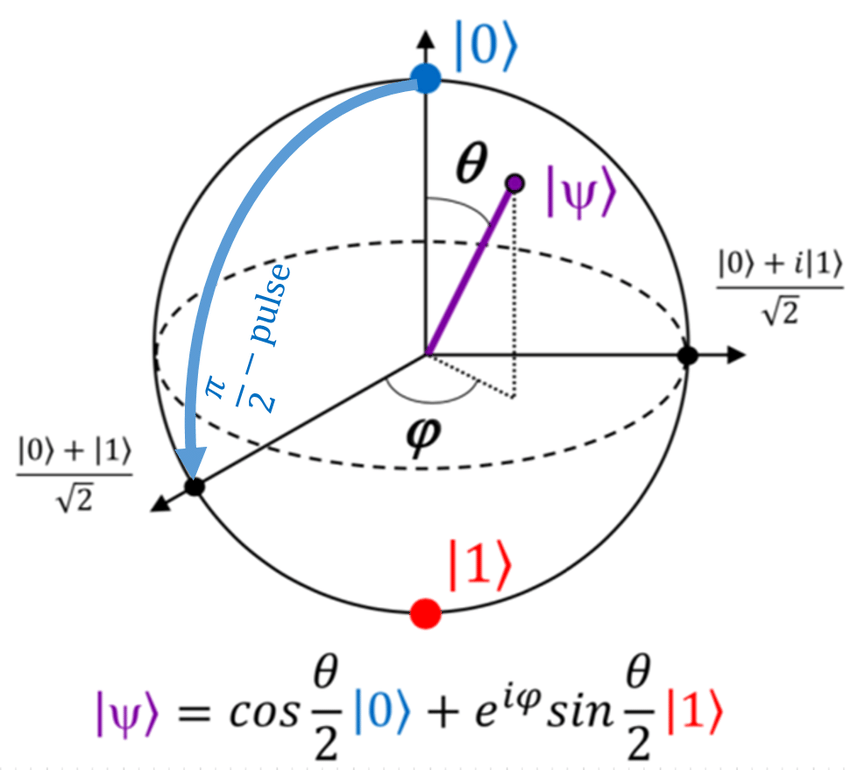
\includegraphics[width=0.5\textwidth]{img/esfera-bloch-diagrama.png}
    \caption{Diagrama da Esfera de Bloch.} 
    \vspace{0.25cm}
    \footnotesize Fonte: A Review on Quantum Computing: Qubits, Cryogenic Electronics and Cryogenic MOSFET Physics.
\end{figure}

Na física rigorosa, a taxa de decoerência é caracterizada pelos tempos de relaxação $T_1$ (tempo de decaimento da energia do qubit) e $T_2$ (tempo de coerência de fase). A probabilidade de erro em uma operação de duração $\tau$ é aproximada por $ P_{erro} = \frac{\tau}{T_1} $. O presente trabalho usa um modelo geométrico simplificado para visualizar esse fenômeno através do Cálculo, os adendos acerca dessa simplificação são descritos na próxima seção.